\documentclass[../main]{subfiles}
\begin{document}

\section{Qualità di processo}
Per parlare della qualità di processo si può cominciare con una semplice frase: "\textit{Da tubi sporchi non esce acqua pulita}". Nel caso dell'\g{ingegneria del software}, i tubi sono i \g{processi} mentre l'acqua è il \g{prodotto software}.\newline
Da questo concetto nasce l'esigenza di evitare che i \g{processi} siano "sporchi", ovvero di scarsa qualità. La qualità di processo, e la sua verifica, devono far parte del ciclo di miglioramento continuo.\newline
\begin{figure}[h]
    \begin{center}
        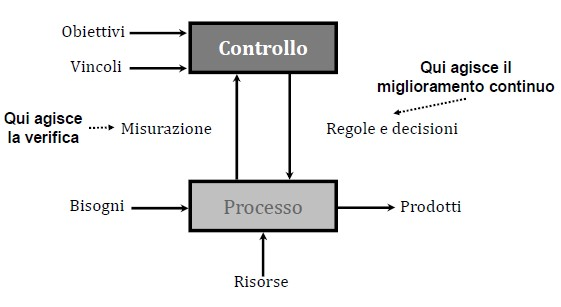
\includegraphics[scale=0.8]{immagini/processo.jpg}
    \end{center}
\end{figure}
Il miglioramento continuo è necessario per migliorare costantemente i \g{processi} e il \g{way of working}, anche se comunque è bene che quest'ultimo sia già buono in partenza (ispirato da standard e \g{best practice}) per i processi primari. La \g{verifica} deve essere continua e quantitativa.
\subsection{Come garantire la qualità di processo?}
Innanzitutto, è bene definire il processo di cui garantire la qualità, in modo da poterlo poi attuare e controllare. Il controllo in questione deve essere fatto:
\begin{itemize}
    \item Sull'\g{efficacia}, per avere prodotti conformi alle attese;
    \item Sull'\g{efficienza}, per utilizzare minori risorse a pari qualità di prodotto;
    \item Sull'esperienza, per permettere di riutilizzare la conoscenza e l'esperienza altrui;
    \item Scegliendo buone metriche che permettano una misurazione quantitativa delle precedenti.
\end{itemize}
\subsection{Standard di qualità di processo}
Per la qualità di processo esiste una famiglia di standard molto conosciuta, che è la ISO 9000. Di queste, la norma ISO 9001 è quella più ambita generalmente nell'industria perché garantisce di essere un fornitore di qualità.
Evoluzione:
\begin{itemize}
    \item ISO 9001:1994 era lo standard per valutare i fornitori;
    \item ISO 9000:2005 elencava modelli di qualità neutri, ovvero validi per più domini applicativi,
    \item ISO 9001:2000, la versione aggiornata del precedente, migliora la definizione del \g{sistema di qualità} e entra più in dettaglio dei sistemi produttivi;
    \item ISO 9000-3:1997 è stato ideato per l'applicazione dello standard ISO 9001:1994 nell'ambito dell'\g{ingegneria del software};
    \item ISO 90003:2014 sostituisce il precedente ISO 9000-3, adattandosi alla nuova versione dello standard ISO 9001:2008;
    \item ISO 9004:2018 ulteriore aggiornamento dello standard, neutro al dominio.
\end{itemize}
\subsection{Principi di un sistema di qualità}
\begin{itemize}
    \item Orientamento al cliente;
    \item Leadership;
    \item Coinvolgimento del personale;
    \item Approccio per processi (in cui è confluito anche l'approccio sistemico alla gestione);
    \item Miglioramento (continuo non è necessario dirlo, perché deve essere necessariamente continuo);
    \item Decisioni basate su evidenze (o dati di fatto);
    \item Gestione delle relazioni.
\end{itemize}
\subsection{Processi di valutazione}
\begin{itemize}
    \item SW Process Assessment \& Improvement (SPY), per la valutazione dei processi di un'organizzazione;
    \item Capability Maturity Model (CMM), poi CMM Integration (CMMI), per la valutazione dei fornitori (inizialmente commissionato dal DoD americano al SWE Institute - SEI);
    \item Software Process Improvement Capability dEtermination (SPICE), che cerca di integrare SPY con ISO/IEC 12207 e ISO 9001, poi confluito in ISO/IEC TR 15504:1998;
\end{itemize}
\subsubsection{SPY}
L'idea alla base dello SPY è quella di avere un processo di valutazione dei \g{processi} di \g{progetto}, la cui valutazione è atta a misurare la loro qualità e a fornire un grado indicativo per facilitare il miglioramento e introdurre modifiche.
\subsection{CMMI}
\begin{itemize}
    \item Capability: misura l'adeguatezza di un processo per gli scopi assegnati che determina una parte della valutazione finale;
    \item Maturity: quanto bene l'azienda governa i suoi processi, la cui valutazione corrisponde alla minima fra tutte quelle ottenute.
    \item Model: insieme di criteri per valutare la qualità dei processi;
    \item Integration: architettura di integrazione dei diversi ambiti (hardware, software, sistema)
\end{itemize}
Riguardo la capability, se il processo ne ha un:
\begin{itemize}
    \item Basso livello, è probabile che esso venga definito e attuato in modo opportunistico e perciò è difficile controllarne l'esito, l'avanzamento e la qualità, portando necessariamente a compromessi in termini di funzionalità e qualità;
    \item Alto livello, è indice che esso viene seguito in modo \g{sistematico}, \g{disciplinato} e \g{quantificabile};
\end{itemize}
L'intelligenza alla base dei processi di un'organizzazione si chiama \g{governance}, ha un'orizzonte aziendale a differenza del \g{management} che ha orizzonte progettuale, e si riferisce al sapere il motivo delle proprie scelte e perché sono efficaci ed efficienti nel proprio ambito aziendale, perché sono best practice e come si relazionano con la visione futura.
\subsubsection{I cinque livelli di maturità}
\begin{figure}[h]
    \begin{center}
        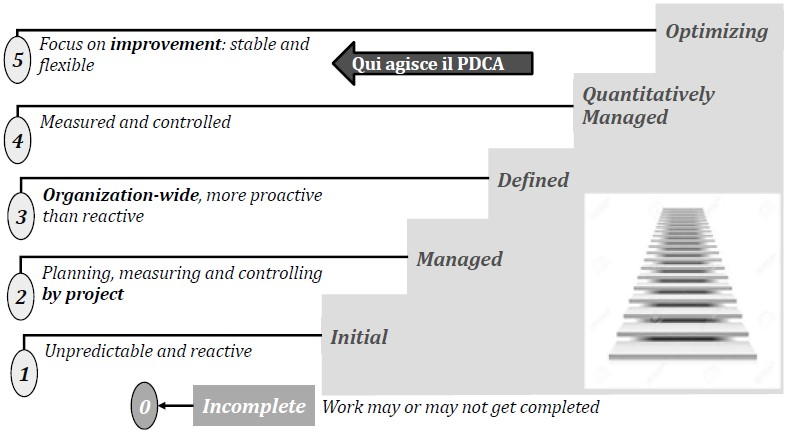
\includegraphics[scale=0.8]{immagini/maturita.jpg}
    \end{center}
\end{figure}
Per comprendere meglio questi cinque livelli si può paragonarlo, ad esempio, alla necessità di spostarsi per raggiungere un luogo.
\begin{figure}[h]
    \begin{center}
        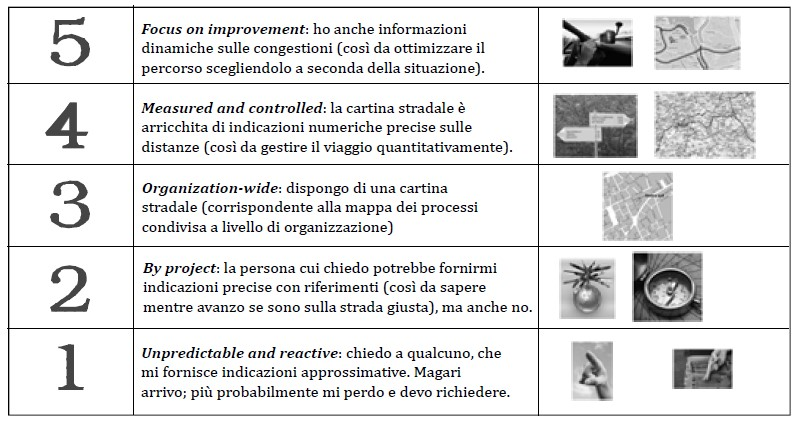
\includegraphics[scale=0.8]{immagini/navigazione.jpg}
    \end{center}
\end{figure}
\end{document}